\chapter{Ergebnisse}

\section{Evaluation der Anwendung}
Alle funktionalen Anforderungen sind im Prototyp der Anwendung in Javascript mit dem node.js-Framework und dem socket.io-Websocket (Abschnitt \ref{socket.io-Server} und \ref{socket.io-Client}) vollständig umgesetzt. Im Screenshot des Hamburger Hafens (Abb. \ref{Hafen Hamburg}) kann man erkennen, dass liegende Schiffe als Kreise dargestellt werden und fahrende Schiffe als Richtungsdreiecke. Wurden Masse übermittelt (AIS-Nachricht vom Typ 4), sind maßstabsgetreue Polygone eingezeichnet, deren Farbe den Schiffstyp kennzeichnet.
Ein Popup mit Detailinformationen zum dem Schiff links daneben ist geöffnet. In dieser Zoomstufe ist die Animation bereits aktiv, das heißt für den Betrachter, dass alle angezeigten Richtungsdreiecke ununterbrochen in Bewegung sind.

\begin {figure}[H]
\begin{center}
  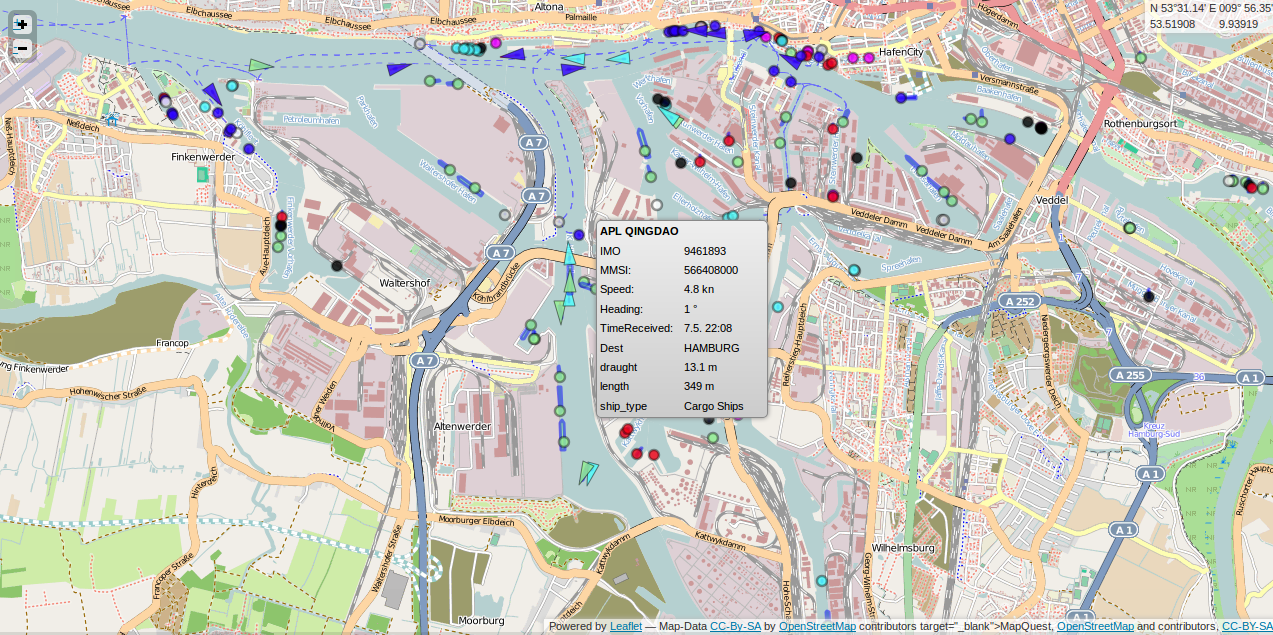
\includegraphics[width=6in]{images/Hamburg.png}
\end{center}
\caption{Anzeige aller Schiffe im Hamburger Hafen}
\label{Hafen Hamburg}
\end {figure}
Das zweite Beispiel zeigt die Situation bei niedriger Zoomstufe (Abb. \ref{Nordsee}). Oben links in der Karte ist ein Hinweis eingeblendet, dass nur Schiffe mit einer Geschwindigkeit über 12 Knoten angezeigt werden. Die Verteilung des Schiffsverkehrs lässt sich gut erkennen, während die große Zahl hafenliegender Schiffe ausgespart bleibt, um die Performance des Browser-Clients zu erhalten. Aus demselben Grund ist die Animation ausgeschaltet. Durch die große Anzahl empfangener Positionsmeldungen, ist die Darstellung trotzdem bewegt.

\begin {figure}[H]
\begin{center}
  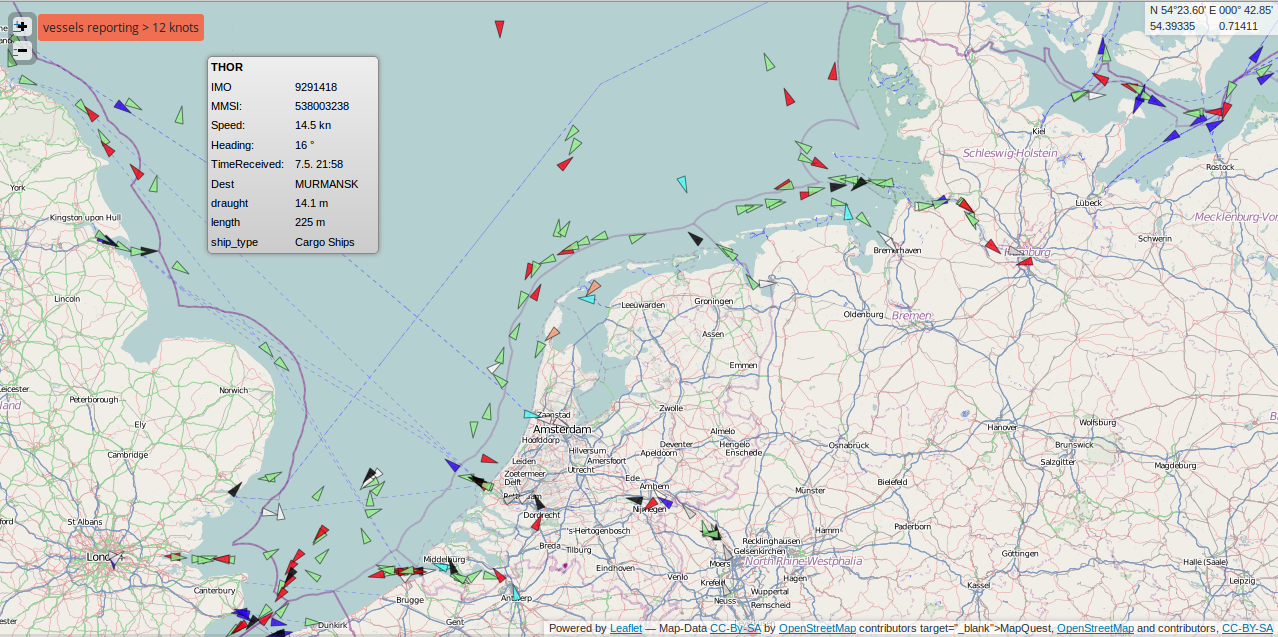
\includegraphics[width=6in]{images/zoomout.png}
\end{center}
\caption{Auf schnell fahrende Schiffe reduzierte Anzeige am Beispiel der Nordsee}
\label{Nordsee}
\end {figure}

\begin {wrapfigure}[9]{r}{3in}
\begin{center}
  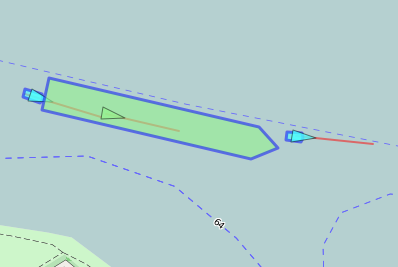
\includegraphics[width=2in]{images/Schleppen.png}
 \caption{Schleppmanöver}
  \end{center}
 \label{Schleppmanöver}

\end {wrapfigure}


Schließlich ist in hohen Zoomstufen eine Beobachtung von aktuellen Schiffsmanövern möglich, wie im Beispiel \ref{Schleppmanöver} das Schleppen eines Frachtschiffes durch zwei Schleppschiffe. Durch die hohe Frequenz der Positions-Meldungen bei fahrenden Schiffe und mithilfe der eingebauten Animation erlebt der Betrachter die Szene wie in einem Animationsfilm.\\

Mit dieser Implementierung wurde auch die wichtige nicht funktionale Anforderung nach einer zeitnahen Umsetzung erfüllt. Der Prototyp wird auf github als privates Repository gehostet und konnte nach der Übergabe (Ende Januar) vom Unternehmen vesseltracker für Weiterentwicklungen der Webanwendung und Kundenprojekte verwendet werden. 
Desweiteren ist die gesamte Anwendung mit open source Produkten entwickelt worden und verwendet das von vom Unternehmen gehostete Kartenmaterial.\newline
Die Latenzzeit zwischen dem Empfang der AIS-Positions-Meldung durch den Rohdatenserver und der Propagierung derselben Position auf der Karte sollte unterhalb 500 msec liegen. 
\begin {wraptable}{r}{3in}
\begin{center}
\begin{tabular}{| l|r|}\hline
& [msec]\\\hline
Mittelwert & 237 \\
Maximum & 701\\
Minimum & 23\\\hline
\end{tabular}
\caption[Latenzzeit von Positionsmeldungen]{Latenzzeit von\\ Positionsmeldungen}
\label{Latenzeit}
\end{center}
 \end {wraptable}
Untersucht wurde die Latenzzeit anhand der ‘time\_received’, die Bestandteil jeder AIS-JSON-Message ist. Dieser Zeitstempel wird vom Rohdatenserver jeder AIS-Message hinzugefügt. Auf dem Rohdatenserver läuft ein ntp-Daemon zur Zeitsynchronisation. Ebenso ein Daemon wurde auf dem Client, auf dem der Browser läuft gestartet und ein Zeitstempel genommen, nachdem das Schiff mit der neuen Position auf die Karte gerendert wurde. Weil die Latenzzeit direkt abhängig ist von der Anzahl der Meldungen, die pro Zeit vom Client emfangen werden, wurde als Referenz eine Ansicht des Hamburger Hafens gewählt in Zoomstufe 12, der niedrigsten Zoomstufe, in der noch Schiffe jeder Geschwindigkeit angezeigt werden. Die Ergebnisse (Tabelle \ref{Latenzzeit}) liegen mit dem Mittelwert gut innerhalb der geforderten Geschwindigkeit.

Die Anzahl der Verbindungen, die der Server gleichzeitig bedienen kann, ist mit einem node.js-Script getestet worden, das alle 500 ms eine neue Clientverbindung erstellt, bis 750 Clients verbunden sind. Der Aufbau der Verbindung geschah auch mit steigender Verbindungsanzahl zuverlässig, jedoch ist in der Abbildung erkennbar, dass die Anzahl der Fälle zunimmt, in denen ein Client lange auf Antwort warten muss.
\\Eine Skalierung der Serveranwendung ist seitens des socket.io-Servers kein Problem. Statt einen einzigen Worker-Prozess zu generieren, können auch mehrere Worker-Prozesse parallel gestartet werden, die alle dieselbe mongo-Datenbank-Collection abfragen und sich bei derselben redis-Datenbank im Channel ‘positionUpdate’ registrieren können. Allerdings muss sichergestellt sein, z.B.  über unterschiedliche Ports oder unterschiedliche (virtuelle) Server, dass ein verbundener Client mit jedem neuen Request auf demselben Worker-Prozess landet.

\begin{figure}[H]
\begin{minipage}[hbt]{3in}
	\centering
	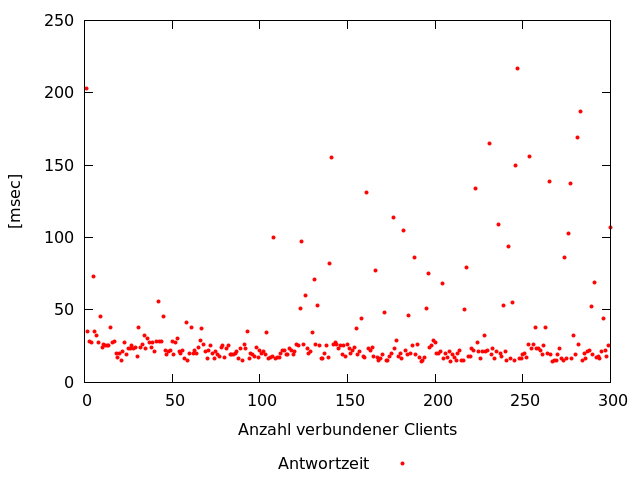
\includegraphics[width=2.5in]{images/stresstest300.png}
	\label{Stresstest300}
\end{minipage}
\hfill
\begin{minipage}[hbt]{3in}
	\centering
	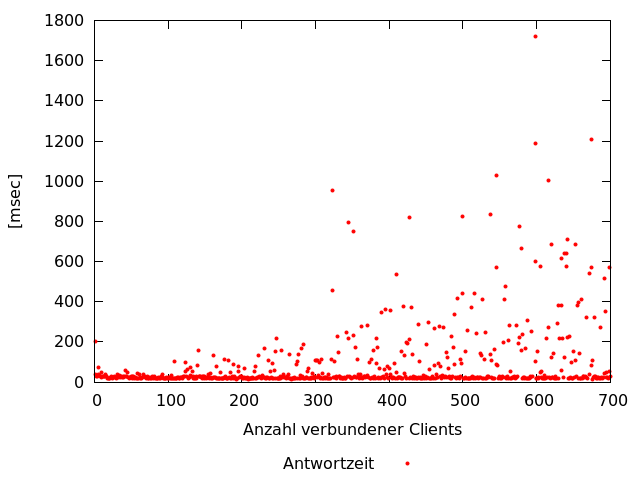
\includegraphics[width=2.5in]{images/stresstest.png}
	\label{Stresstest}
\end{minipage}
\caption{Anwortzeiten des socket.io-Websocket-Servers in Abhängigkeit von der Anzahl verbundener Clients}
\end{figure}
%-------------------------------------------------------------------------------------------------------------------------------------------
\section{Vergleichende Evaluation der Javascript- und der Dart-Anwendung}
Die in Google Dart geschriebene Client-Anwendung soll nun mit dem in Javascript programmierten Client verglichen werden. Die in den Abschnitten  \ref{Strategie-Korrektur} und \ref{Vergleichbarkeit} begründete zusätzliche Implementierung eines HTML5-kompatiblen node.js-Websocket-Servers muss nun in einem ersten Schritt mit dem node.js-socket.io-Server verglichen werden. Für diesen und alle folgenden Tests wurde auf dem Rohdatenserver ein Port eingerichtet, der nur die Daten von drei AIS-Antennen (Hamburg, Wedel, Geesthacht) ausgibt. Dies war notwendig, um den als Server verwendeten Arbeitsplatzrechner (MHz und 1 GB Arbeitsspeicher) nicht zu überlasten. Dadurch entstünde eine zusätzliche Latenzzeit wegen des kontinuierlichen Anwachsens der Messagequeues auf dem Server, die die Ergebnisse verzerrt.
\subsection{Node.js - socket.io-Socket-Server vs. node.js-Websocket-Server}\label{socket.io- vs html5-Server}
\subsubsection{Implementierungsaufwand}
Im Implementierungsaufwand unterscheiden sich beide Server- und Client-Anwendungen kaum (Anzahl zeilen code).  Einige Features der socket.io-Bibliotheken (z.B. die Clientverwaltung, Parameter für ‘Production’ und ‘Development’-Umgebung bezüglich Logleveln, Client-minification oder Client-Zip) sind praktisch und müssten in der Alternativimplementierung für den Einsatz in einer produktiven Umgebung anderweitig gelöst werden. Durch die in socket.io eingeführten Events vermindert sich der Kommunikationsaufwand zwischen Server und Client geringfügig, was in diesem Fall einer datenintensiven Anwendung mit großen Datenmengen pro Nachricht wenig zu Buche schlägt.
\subsection{Latenzzeit}
Die Leistungsfähigkeit beider Implementierungen wird verglichen, indem wieder wie in Tabelle \ref{Latenzzeit} die Zeit gemessen wird, die eine Positionsmeldung braucht für den Weg vom Rohdatenserver bis zur Präsentation auf der Karte. Um eine ähnliche Situation in beiden Szenarien abzubilden, wurde jeweils eine bestimmte Position in Hafen Hamburg angesteuert und ein Timer in die Client-Anwendung integriert, der jeweils nach einer Minute um eine Stufe herauszoomt. Da ab Zoomlevel 11 und kleiner nur noch Schiffe mit einer jeweils definierten Mindestgeschwindigkeit angezeigt werden, nahm die Anzahl empfangener Schiffe von dieser Zoomstufe an wieder ab. Zur Auswertung wird auf dem Client ein LogFile geschrieben, das pro Nachricht, deren ‘time\_received’ und einen aktuellen Zeitstempel schreibt.  Die Differenz wird als Latenzzeit interpretiert. Anschließend wird über das Logfile berechnet, wieviele Positionsmeldungen in einer Minute an den Client gesendet wurden. Darüber ist es möglich, die Latenzzeit gegen die Anzahl empfangener Positionsmeldungen pro Minute darzustellen, wie in Abbildung \ref{Latenzzeit socket.io} und \ref{Latenzzeit HTML5} zu sehen.
\begin {figure}[H]
\begin{center}
  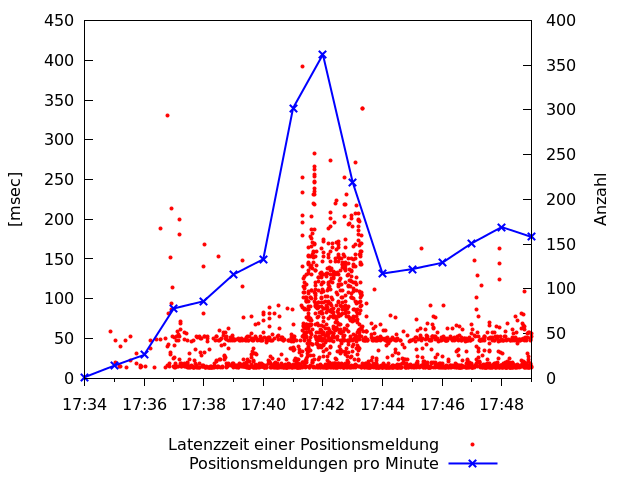
\includegraphics[width=4.5in]{images/latency_timeReceived_socket_io.png}
\end{center}
\caption{socket.io-Websocket-Server: Latenzzeit der Positionsmeldungen und Anzahl empfangener Schiffe}
\label {Latenzzeit socket.io}
\end {figure}

\begin {figure}[H]
\begin{center}
  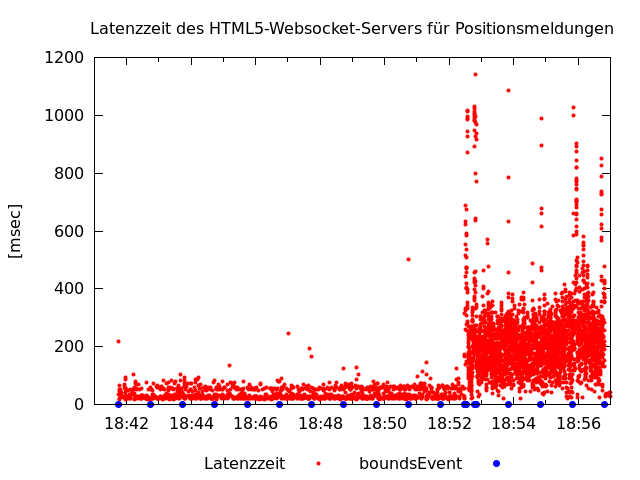
\includegraphics[width=4.5in]{images/latency_timeReceived_HTML5.png}
\end{center}
\caption{HTML5-Websocket-Server: Latenzzeit der Positionsmeldungen und Anzahl empfangener Schiffe}
\label {Latenzzeit HTML5}
\end {figure}
Es ist offensichtlich, dass die Geschwindigkeit in der Darstellung von der Anzahl empfangener Nachrichten linear abhängt.
Darüber hinaus ist zu erkennen, dass beide Implementierungen ihre Aufgabe in ähnlicher Geschwindigkeit erledigen. 

\subsection{Browserunterstützung}
Firefox, Chrome, IE, Safari


\section{Javascript-Client vs. Dart-Client} 
\subsection{Implementierungsaufwand}
In der Dart-Implementierung verlangt das Arbeiten mit zwei unterschiedlichen Scopes (javascript und Dart) dem Programmierer einiges ab und ist am Anfang sehr fehleranfällig. Die Fehler sind schwierig zu debuggen, weil der Debugger (javascript-Debugger Firebug oder der Debugger im DartEditor) ebenfalls nicht über die Grenzen des Namensraumes wechseln können. 

\subsection{Performance}
Um die unterschiedliche Performance des Javascript- und des Dart-Clients zu vergleichen, wurde der VesselInBounds-Event genutzt. Gemessen wurde die Zeit, die benötigt wird, um nach Empfang eines VesselInBounds-Events alle in der Message enthaltenen Schiffe auf die Karte zu rendern. Dazu wurden die Browser Dartium, Chrome und Firefox auf dem Client benutzt.
\begin{itemize}
\item in Google Dartium wird bei Aufruf des Dart-Clients der originäre Dart-Code interpretiert. Beim Aufruf des Javascript-Clients wird der Javascript-Code interpretiert.
\item in Google Chrome wird bei Aufruf des Dart-Clients der mit dart.js zu javascript kompilierte Dart-Code interpretiert und beim Aufruf des Javascript-Clients der Javascript-Code mit der V8-Engine.
\item in Firefox
\end {itemize}
\newpage

\begin {figure}[H]
\begin{center}
  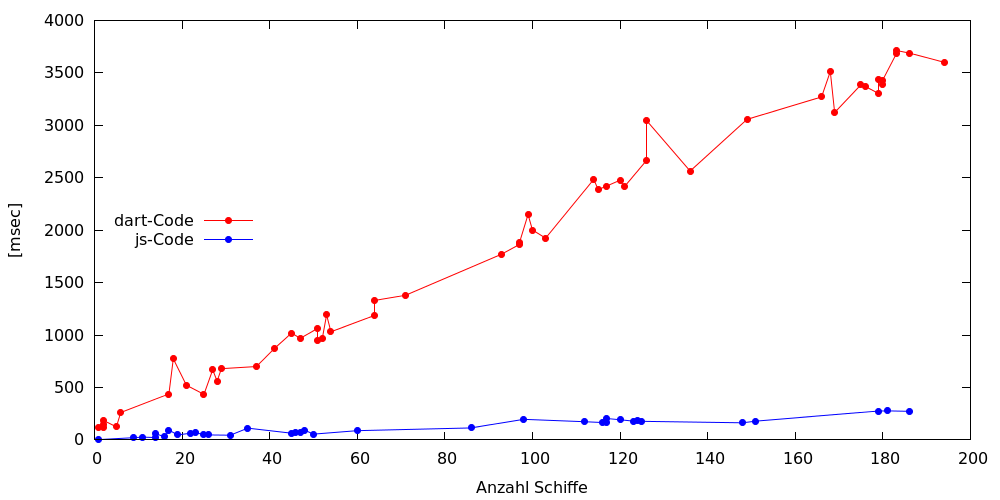
\includegraphics[height=2.3in]{images/Dartium.png}
\end{center}
 \caption{Dauer des Renders in Dartium}
\end {figure}


\begin {figure}[H]
\begin{center}
  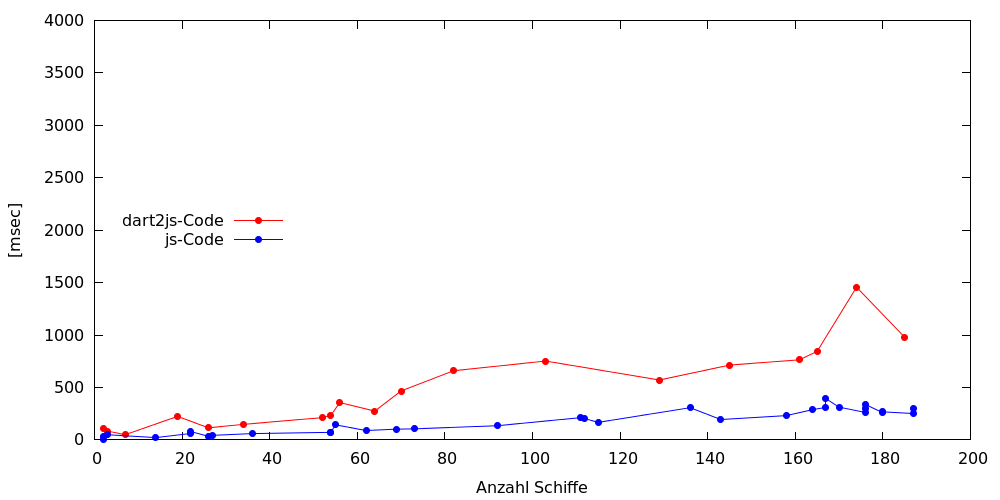
\includegraphics[height=2.3in]{images/Chrome.png}
\end{center}
 \caption{Dauer des Renders in Chrome}
\end {figure}


\begin {figure}[H]
\begin{center}
  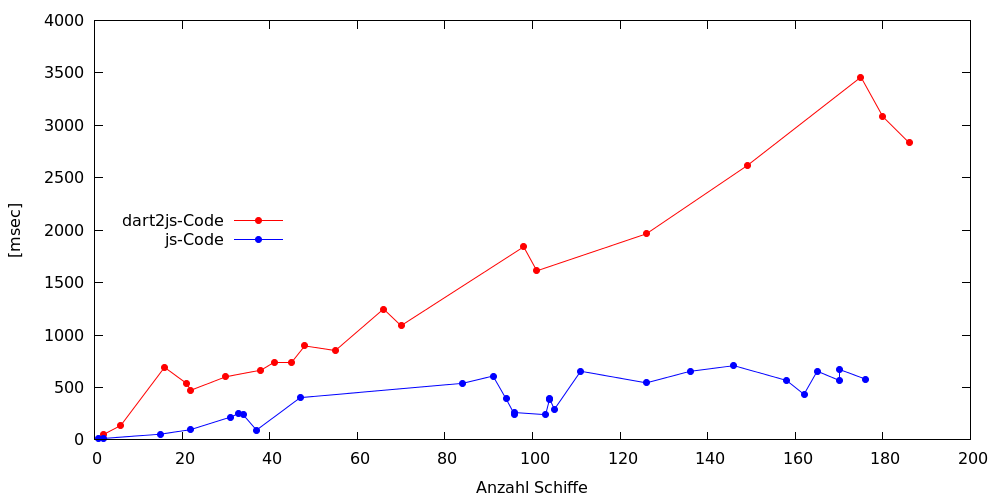
\includegraphics[height=2.3in]{images/Firefox.png}
\end{center}
 \caption{Dauer des Renders in Firefox}
\end {figure}


\subsection{Browserunterstützung}
\subsubsection{Dartium}

\subsubsection{Firefox, Chrome, IE, Safari}

Der dart-Client kompiliert den in Dart geschriebenen Code zu Javascript.

Dabei traten Fehler auf, die unter Dartium (also im originalen Dart-Code) nicht auftraten.
1. Wird innerhalb des Javascript-Scopes eine Methode auf einen javascript-Proxy (hier \_map) aufgerufen und ein proxy wird zurückgegeben, dann ist es nicht möglich auf diesen Proxy, der in diesem Fall vom Typ LatLngBounds sein müsste, eine Methode der Klasse LatLngBounds aufzurufen. => TypeError: t1.get\$\_map(...).getBounds\$0(...).getSouthWest\$0 is not a function

dart-client: web/leaflet\_maps.dart

  List getBounds(){
    var south, west, north, east;
    js.scoped((){
    south= \_map.getBounds().getSouthWest().lng;
        west = \_map.getBounds().getSouthWest().lat;
        north = \_map.getBounds().getNorthEast().lng;
        east = \_map.getBounds().getNorthEast().lat;
 });
return [west, south, east, north];
    
In diesem Fall wird einfach als work-Around eine andere Methode verwendet (getBBoxString), die einen String mit den Bounds zurückgibt. Aus den Teilen dieses Strings werden mit der Methode parse(string) der Klasse double die Werte der Eckpunkte der Bounds generiert.

String getBounds(){
    String bBox;
    js.scoped((){
      bBox = \_map.getBounds().toBBoxString();
    });
    return bBox;
  }

 Weil dadurch der message-Parameter 'bounds' kein number-Array, sondern ein String ist, muss im html5-Server der String einmal zum Float geparst werden.



2. Ein Feld ("IMO") wird auf null und auf > 0 geprüft.


\chapter{Fazit}\label{Fazit}
 \section{Ergebnisse }
\subsection{Die Realtime-Applikation}


Features, die in die Anwendung integriert werden sollten:
\begin{itemize}
\item eine aufklappbare Liste, in die der Nutzer favorisierte Häfen speichern kann, die dann mit einem Klick angesteuert werden können.
\item eine Legende mit einer Erläuterung der farbigen Schiffssymbole
\item zur weiteren Optimierung der Anwendung, sollte die Möglichkeit, die Animation der Richtungsdreiecke und Schiffspolygon über css3-Transition-Funktionen zu realisieren, unbedingt weiterverfolgt werden
\end{itemize}

\subsection{Vergleich Javascript und Google Dart}
Wie in den Abbildung zur Struktur der Anwendung erkennbar, ist mit Dart sehr viel einfacher Objektorientiertheit herzustellen. Dadurch wird die Anwendung einfacher zu verstehen und damit auch einfacher zu entwerfen, zu schreiben und zu warten.

\section{Ausblick}
Legende
-Satellitendaten in die Anwendung einbinden

